\documentclass[12pt,addpoints]{exam}
\usepackage{enumitem}
\usepackage{amsfonts,amssymb,amsmath, amsthm}
\usepackage{graphicx}
\usepackage{systeme}
\usepackage{pgf,tikz,pgfplots}
\pgfplotsset{compat=1.15}
\usepgfplotslibrary{fillbetween}
\usepackage{mathrsfs}
\usetikzlibrary{arrows}
\usetikzlibrary{calc}\author{St John Baptist De La Salle Catholic School, Addis Ababa}
\usepackage{geometry}
\date{2023}
\geometry{
	a4paper,
	total={170mm,257mm},
	left=15mm,
	right=15mm,
	bottom=20mm,
	top=5mm,
}
\begin{document}
	\title{Grade 11 Physics Workbook}
	\maketitle
	
	\begin{center}
		\section*{Unit 3 - Kinematics}
		\begin{questions}
			\question On a 30 km bike ride, you ride the first 10 km at an average speed of 8 km/hour. What average speed must you have over the next 12km if your average speed for the whole ride is to be 18 km/hour?\vspace{1.3in}
			\question An object starts moving at $t = 0$, and its position is given by $x = At^5 - Bt^2$, where $t$ is in seconds and $x$ is in meters. A is a non-zero constant.
			\begin{enumerate}[label=(\alph*)]
				\item Infer the units of A and B.\vspace{0.8in}
				\item Find the velocity as a function of $t$.\vspace{1in}
				\item What is the average velocity from $0$ to $t$ as a
				function of time?\vspace{1in}
				\item At what time $t$ $(t > 0)$ is the velocity at t
				equal to the average velocity from $0$ to $t$?\vspace{1in}
			\end{enumerate}
			\question You’re standing on the roof of a building, which is 13.0 meters above the ground. You have a rock in your hand, which you can throw with a maximum speed of 12.0 m/s.
			\begin{enumerate}[label=(\alph*)]
				\item How long would it take for the rock to hit the
				ground if you released the rock from rest?\vspace{1in}
				\item How long would it take for the rock to hit the
				ground if you threw the rock straight downward?\vspace{1in}
				\item How long would it take for the rock to hit the
				ground if you threw the rock straight upward?\vspace{1in}
				\item If you threw the rock straight upward, how
				high would it get above the ground?\vspace{1in}
			\end{enumerate}
			\question If the acceleration due to gravity on a planet is $\frac{1}{4}$ that on Earth, how many times longer does it take for a rock to drop the same distance on the planet?\vspace{1.5in}
			\question The graph below represents the motion of a ball that rolls up a hill and then back down. When does the ball return to the location it had at $t = 0$? Also, express the velocity and acceleration as functions of time.
			\begin{center}
				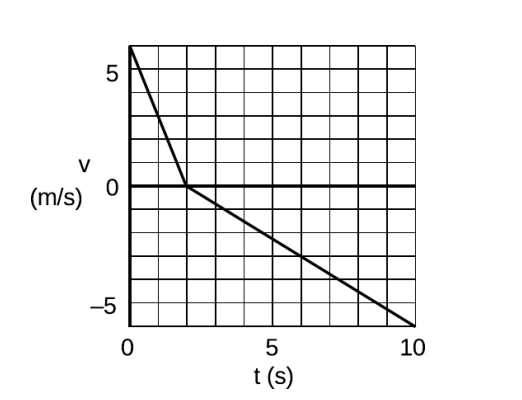
\includegraphics[scale=0.3]{graph1.png}
			\end{center}
			\vspace{1in}
			\question 
			\begin{enumerate}[label=(\alph*)]
				\item Express the chain rule in Leibniz
				(“d”) notation, and show that it always results
				in an answer whose units make sense.\vspace{1in}
				\item An object has a position as a function of
				time given by $x = A\cos(bt)$, where A and b
				are constants. Infer the units of A and b, and
				interpret their physical meanings.\vspace{1in}
				\item Find the velocity of this object, and check
				that the chain rule has indeed given an answer
				with the right units.\vspace{1in}
			\end{enumerate} 
			\question A honeybee’s position as a function of time is given by $x = 10t^2-t^5$, where $t$ is in seconds and $x$ in meters. What is its velocity at $t = 3.0s$?\vspace{1in}
			\question Assume you are an astronaut, and you’ve arrived on some planet P, which has no atmosphere. You drop a hammer from a height of 1.00 m and find that it takes 10ms to fall to the ground. What is the acceleration due to gravity on the planet P?\vspace{1.5in}
			\question Objects A and B, with $v(t)$ graphs shown in the figure, both leave the origin at time $t = 0 s$. When do they cross paths again?
			\begin{center}
				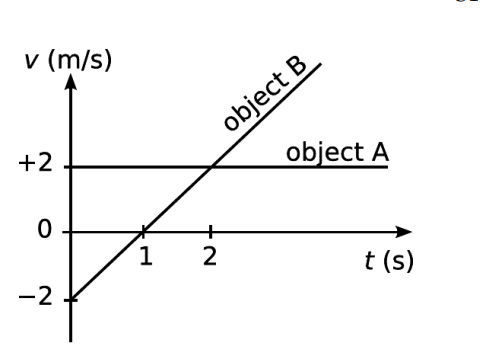
\includegraphics[scale=0.3]{graph2.png}
			\end{center}\vspace{1in}
			\question Starting from rest, a ball rolls down a ramp, traveling a distance L and picking up a final speed $v$. How much of the distance did the ball have to cover before achieving a speed of $\dfrac{v}{2}$?\vspace{1in}
			\question You climb half-way up a tree, and drop a rock. Then you climb to the top, and drop another rock. How many times greater is the velocity of the second rock on impact?\vspace{1in}
			\question Some fleas can jump as high as $30 cm$. The flea only has a short time to build up speed — the time during which its center of mass is accelerating upward but its feet are still in contact with the ground. Make an order-of-magnitude estimate of the acceleration the flea needs to have while straightening its legs, and state your answer in units of g, i.e., how many “g’s it pulls.”(For comparison, fighter pilots black out or die
			if they exceed about 5 or 10 g’s.)\vspace{1in}
			\question A person is parachute jumping. During the time between when she leaps out of the plane and when she opens her chute, her altitude is given by an equation of the form
			$$y=b-c(t+ke^{\frac{-t}{k}}),$$
			where $e$ is the base of natural logarithms, and $b$, $c$, and $k$ are constants. Because of air resistance, her velocity does not increase at a steady rate as it would for an object falling in vacuum.
			\begin{enumerate}[label=(\alph*)]
				\item What units would $b$, $c$, and $k$ have to have for the equation to make sense?\vspace{1in}
				\item Find the person’s velocity, $v$, as a function of time. [Hint: $\dfrac{d e^x}{dx}=e^x$]\vspace{1in}
				\item Use your answer from part (b) to get an interpretation of the constant $c$. [Hint: $e^{-x}$ approaches zero for large values of $x$.]\vspace{1in}
				\item Find the person’s acceleration, $a$, as a function of time.\vspace{1in}
				\item Use your answer from part (d) to show that if she waits long enough to open her chute, her acceleration will become very small.\vspace{1in} 
			\end{enumerate}
		\end{questions}
		

	\end{center}		
\end{document}